% --- Part 4: Redes Neuronales y Cifrado Homomórfico ---
\section{Redes Neuronales y FHE}
\SectionFrame{Redes Neuronales y Cifrado Homomórfico}

\begin{frame}{Operaciones en el espacio cifrado}
    La ejecución de RNAs sobre FHE requiere traducir las operaciones tensoriales al dominio de polinomios:
    \vspace{0.4cm}
    \begin{itemize}
        \setlength{\itemsep}{12pt}
        \item \textbf{Multiplicación Matriz-Vector:} Se realiza mediante la técnica de diagonalización desarrollada por Halevi y Shoup.
        \item \textbf{Convoluciones:} Se transforman en productos matriciales eficientes mediante la técnica \textbf{Im2Col} sobre los datos cifrados.
        \item \textbf{Funciones de Activación:} Dado que FHE solo permite sumas y productos, activaciones como ReLU o Sigmoid se sustituyen por \textbf{aproximaciones polinomiales} (ej. $f(x) = x^2$).
    \end{itemize}
\end{frame}

\begin{frame}{Redes de interés}
    \begin{itemize}
        \item \textbf{Capa Lineal ($y = Wx + b$):} Base de los Perceptrones Multicapa (MLP), resolvemos mediante productos punto paralelos.
        \item \textbf{Capa Convolucional:} Fundamental para visión artificial, procesa regiones espaciales locales.
    \end{itemize}
    \vspace{0.2cm}
    \begin{columns}[t]
        \column{0.45\textwidth}
        \centering
        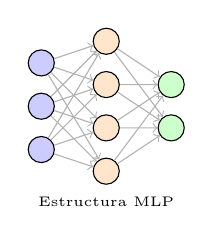
\begin{tikzpicture}[scale=0.55, every node/.style={font=\tiny}]
            % Input layer
            \foreach \i in {1,...,3}
                \node[circle, draw, fill=blue!20] (I\i) at (0,\i) {};
            % Hidden layer
            \foreach \i in {1,...,4}
                \node[circle, draw, fill=orange!20] (H\i) at (1.5,\i-0.5) {};
            % Output layer
            \foreach \i in {1,...,2}
                \node[circle, draw, fill=green!20] (O\i) at (3,\i+0.5) {};
            % Connections
            \foreach \i in {1,...,3}
                \foreach \j in {1,...,4}
                    \draw[->, gray!60] (I\i) -- (H\j);
            \foreach \i in {1,...,4}
                \foreach \j in {1,...,2}
                    \draw[->, gray!60] (H\i) -- (O\j);
            \node[below=0.2cm] at (1.5, 0.5) {Estructura MLP};
        \end{tikzpicture}
        
        \column{0.55\textwidth}
        \centering
        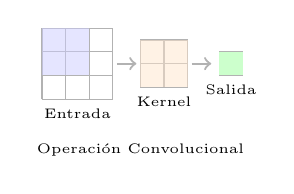
\begin{tikzpicture}[scale=0.5, every node/.style={font=\tiny}]
            % ENTRADA
            \begin{scope}[shift={(0,0)}]
                \draw[step=0.6cm, gray!60, thin] (0,0) grid (1.8,1.8);
                \fill[blue!20, opacity=0.5] (0,0.6) rectangle (1.2,1.8);
                \node[below] at (0.9, 0) {Entrada};
            \end{scope}
            % KERNEL
            \begin{scope}[shift={(2.5,0.3)}]
                \draw[step=0.6cm, gray!60, thin] (0,0) grid (1.2,1.2);
                \fill[orange!20, opacity=0.5] (0,0) rectangle (1.2,1.2);
                \node[below] at (0.6, 0) {Kernel};
            \end{scope}
            \draw[->, thick, gray!60] (1.9, 0.9) -- (2.4, 0.9);
            \draw[->, thick, gray!60] (3.8, 0.9) -- (4.3, 0.9);
            % SALIDA
            \begin{scope}[shift={(4.5,0.6)}]
                \draw[step=0.6cm, gray!60, thin] (0,0) grid (0.6,0.6);
                \fill[green!20] (0,0) rectangle (0.6,0.6);
                \node[below] at (0.3, 0) {Salida};
            \end{scope}
            \node[below=0.2cm] at (2.5, -0.5) {Operación Convolucional};
        \end{tikzpicture}
    \end{columns}
\end{frame}
